ここでは6.3.1で記した, 共振ピークの同定の際に測定した伝達関数(各方向の励起信号からMNの動きまでの伝達関数)を示す. \\\\
\noindent
\underline{{\bf ETMX MN L}}
\begin{figure}[H]
\begin{center}
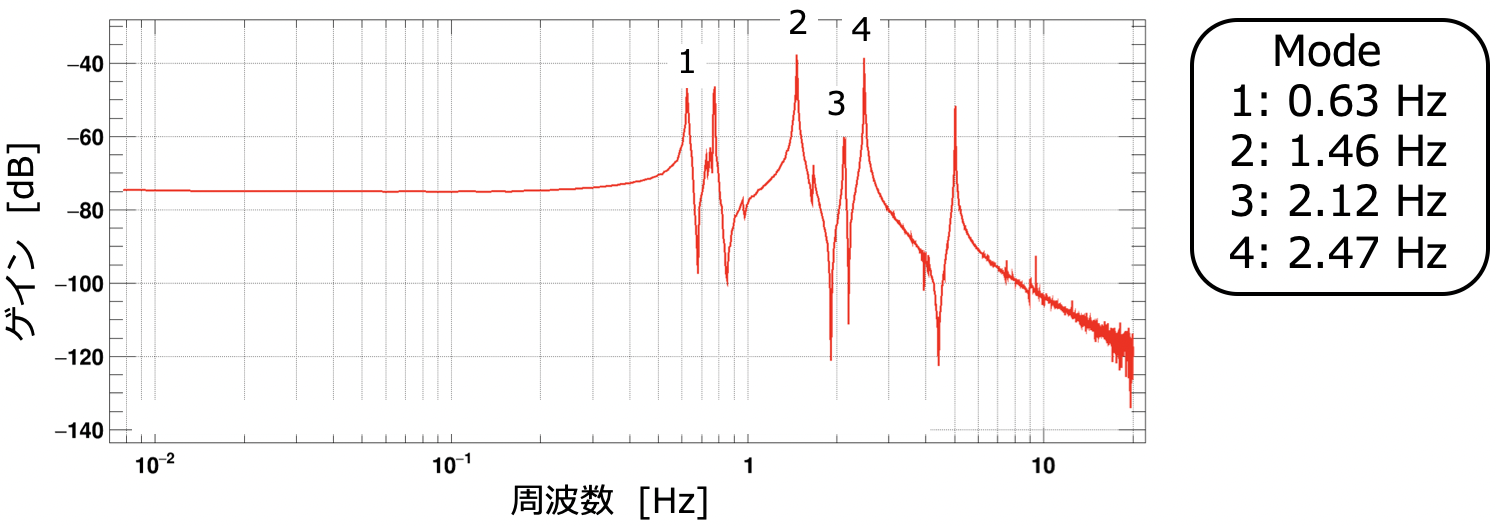
\includegraphics[width=150mm]{figD_1.png}
\end{center}
\end{figure}
\noindent
\underline{{\bf ETMX MN T}}
\begin{figure}[H]
\begin{center}
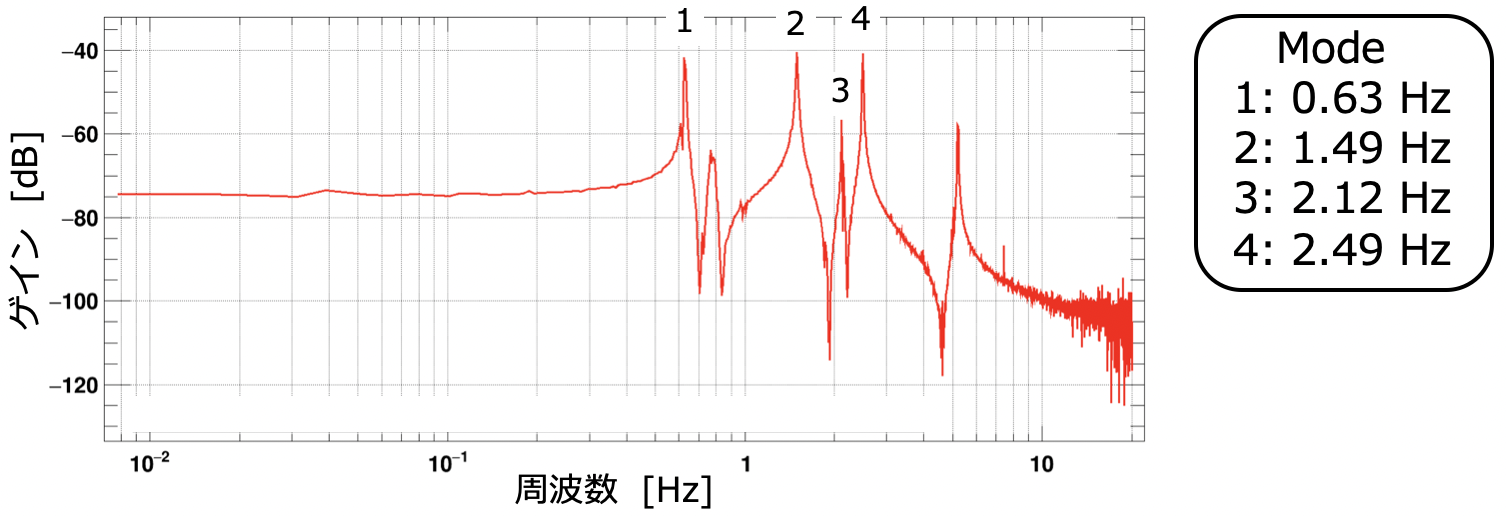
\includegraphics[width=150mm]{figD_2.png}
\end{center}
\end{figure}
\clearpage
\noindent
\underline{{\bf ETMX MN R}}
\begin{figure}[H]
\begin{center}
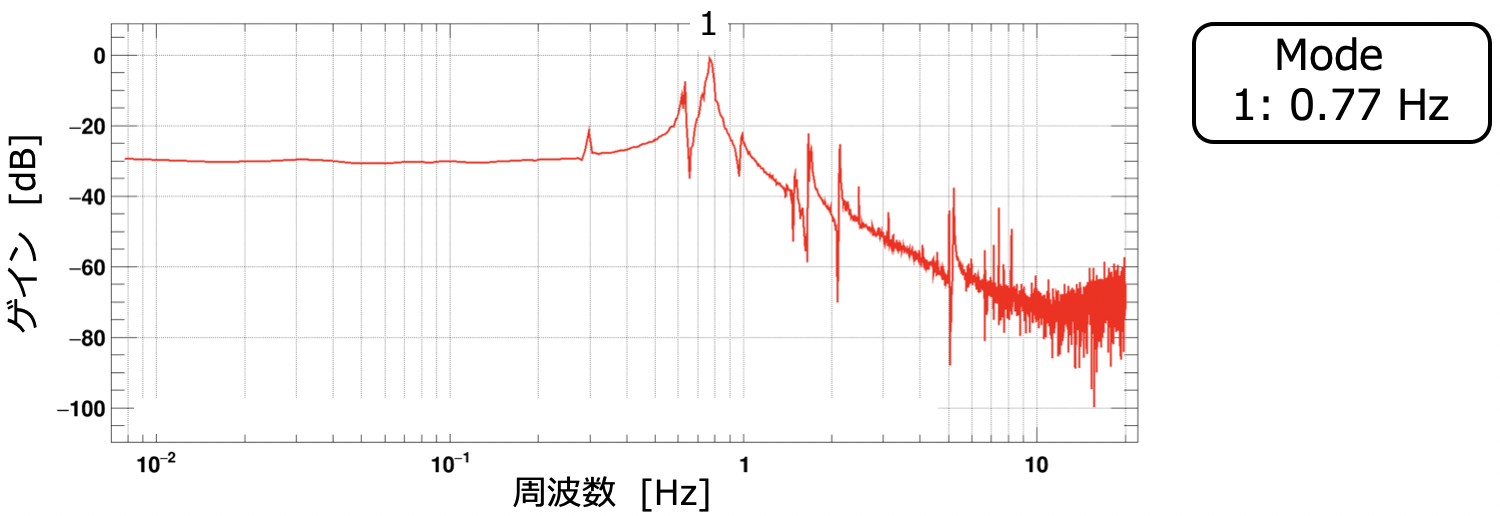
\includegraphics[width=150mm]{figD_3.png}
\end{center}
\end{figure}
\noindent
\underline{{\bf ETMX MN P}}
\begin{figure}[H]
\begin{center}
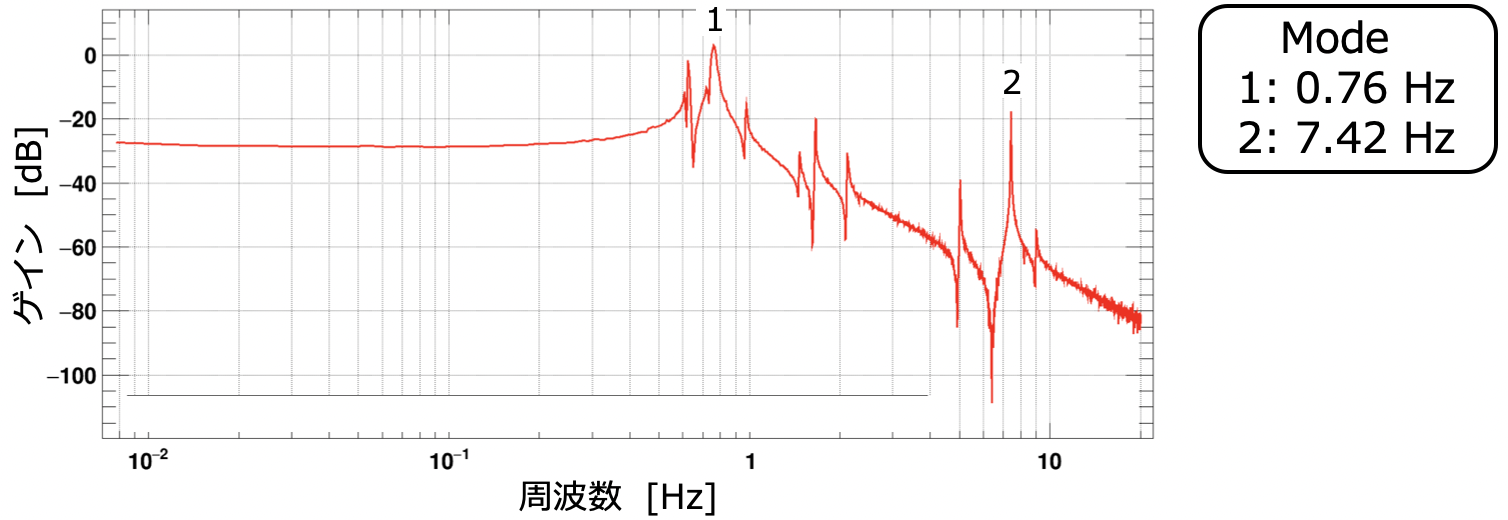
\includegraphics[width=150mm]{figD_4.png}
\end{center}
\end{figure}
\noindent
\underline{{\bf ETMX MN Y}}
\begin{figure}[H]
\begin{center}
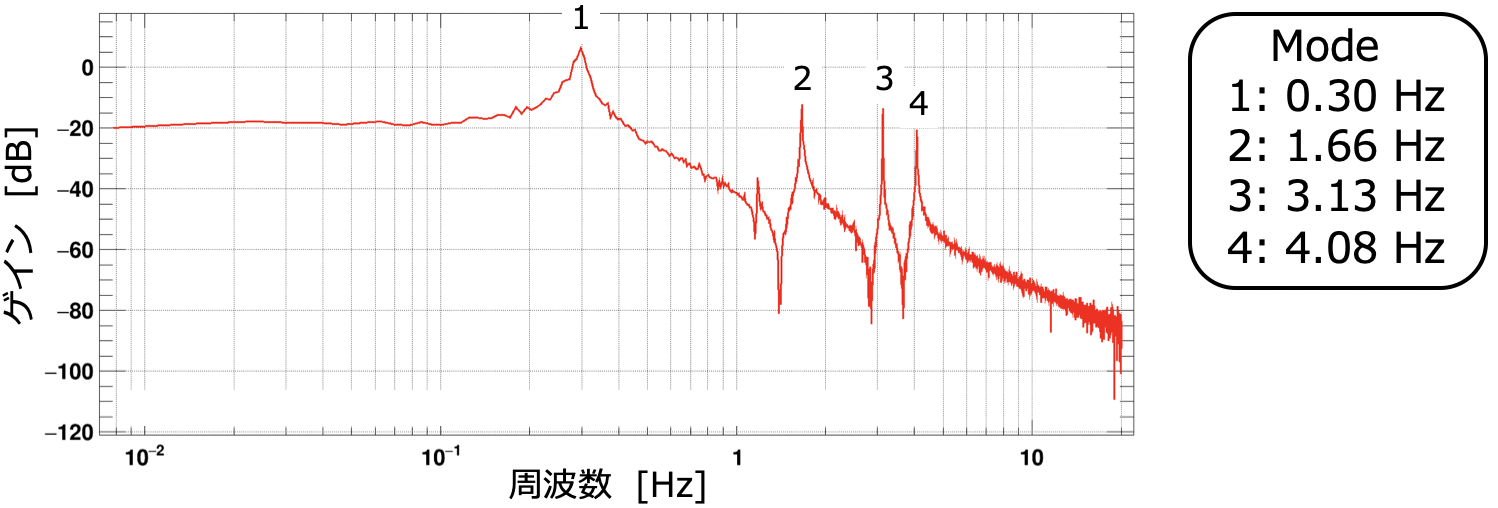
\includegraphics[width=150mm]{figD_5.png}
\end{center}
\end{figure}
\clearpage
\noindent
\underline{{\bf ETMY MN L}}
\begin{figure}[H]
\begin{center}
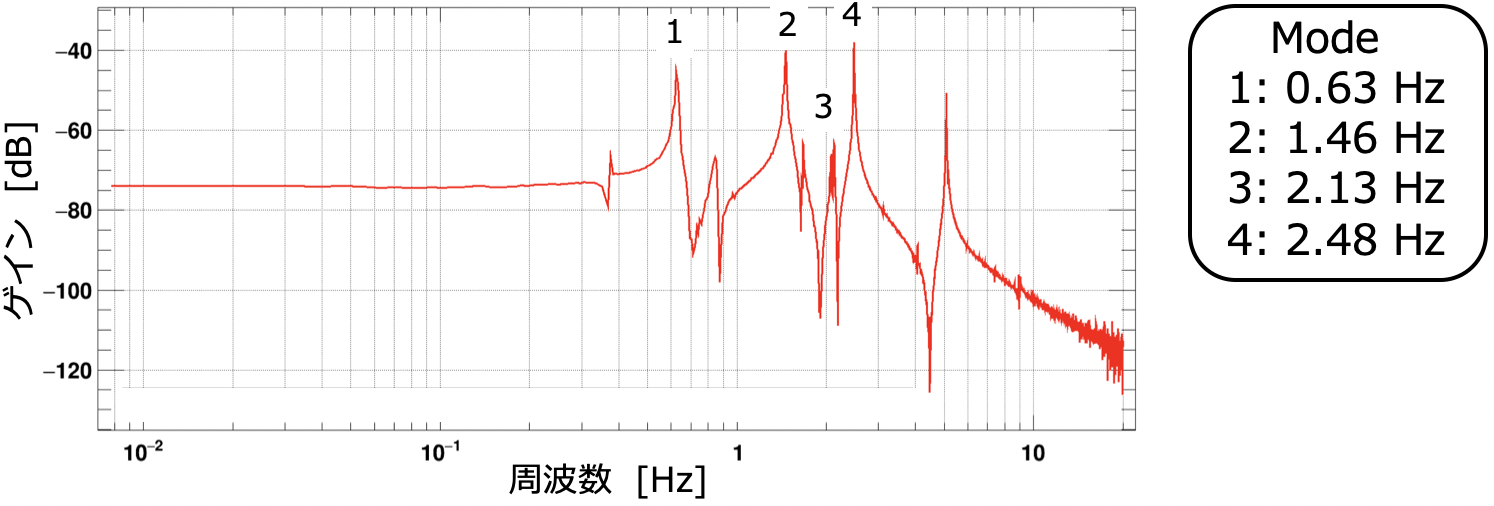
\includegraphics[width=150mm]{figD_6.png}
\end{center}
\end{figure}
\noindent
\underline{{\bf ETMY MN T}}
\begin{figure}[H]
\begin{center}
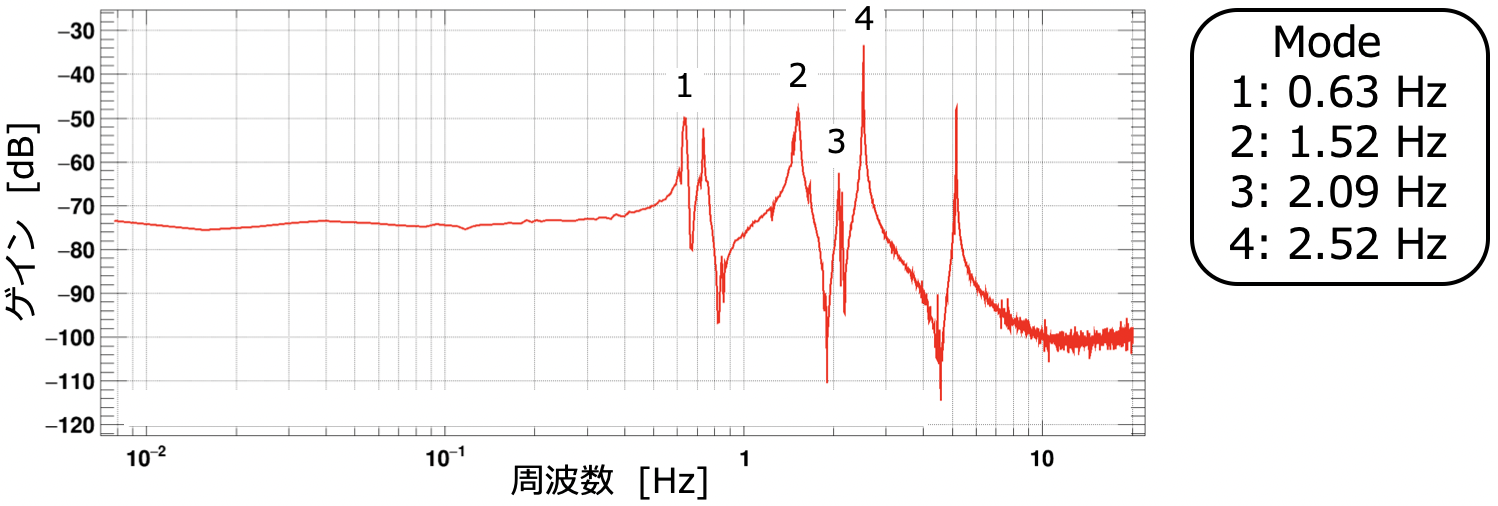
\includegraphics[width=150mm]{figD_7.png}
\end{center}
\end{figure}
\noindent
\underline{{\bf ETMY MN R}}
\begin{figure}[H]
\begin{center}
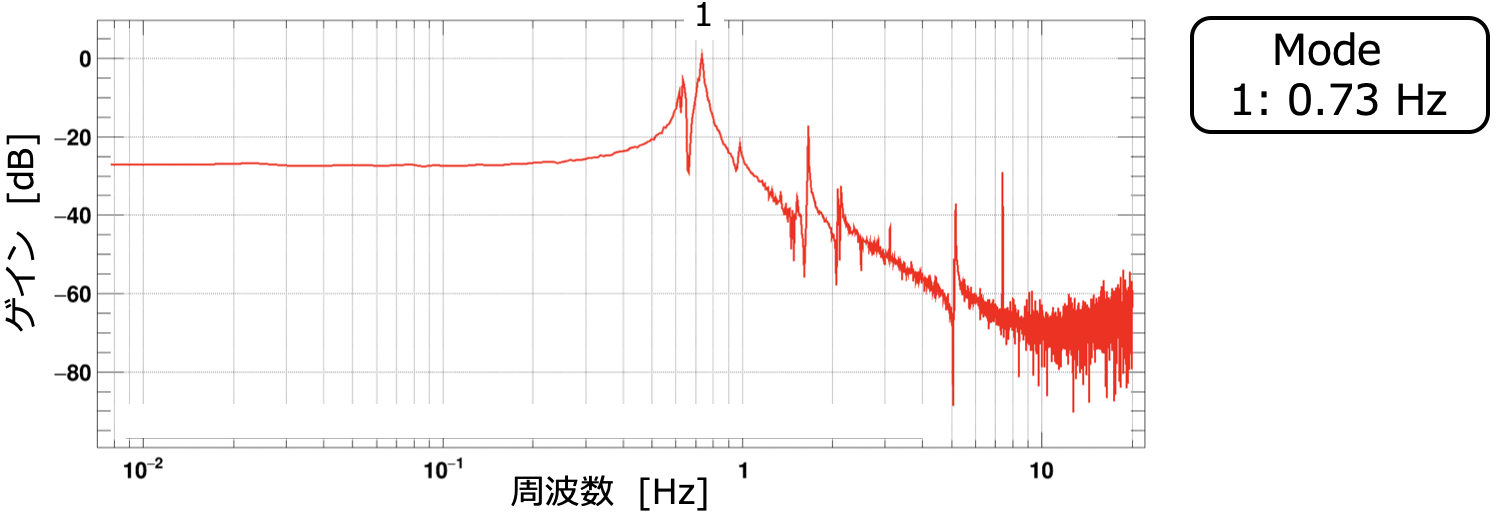
\includegraphics[width=150mm]{figD_8.png}
\end{center}
\end{figure}
\clearpage
\noindent
\underline{{\bf ETMY MN P}}
\begin{figure}[H]
\begin{center}
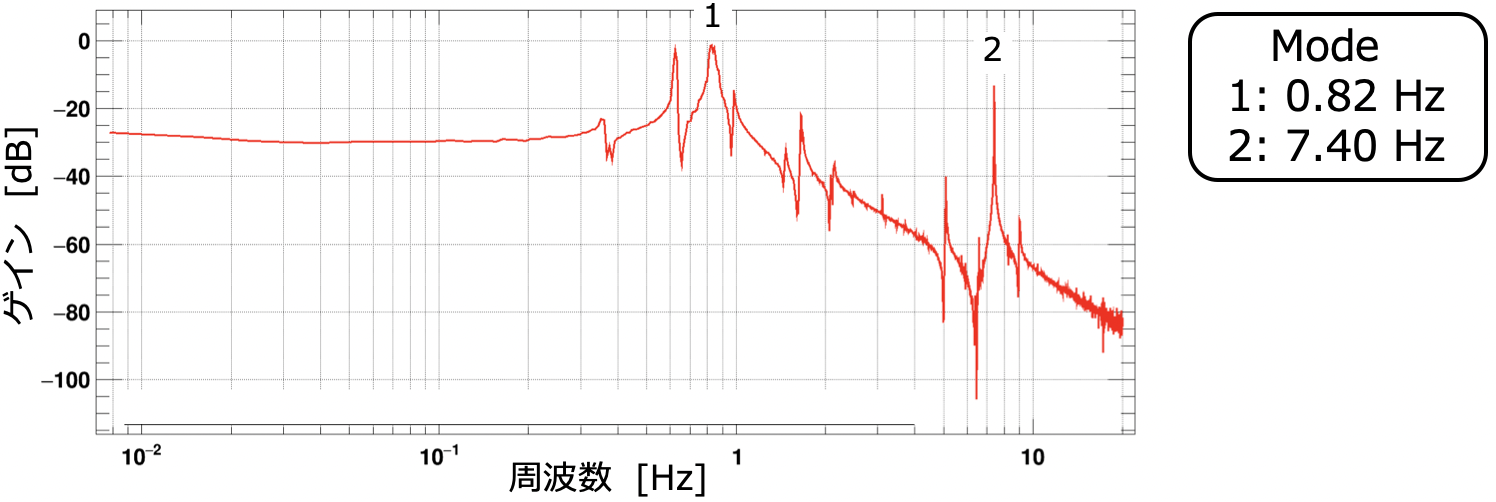
\includegraphics[width=150mm]{figD_9.png}
\end{center}
\end{figure}
\noindent
\underline{{\bf ETMY MN Y}}
\begin{figure}[H]
\begin{center}
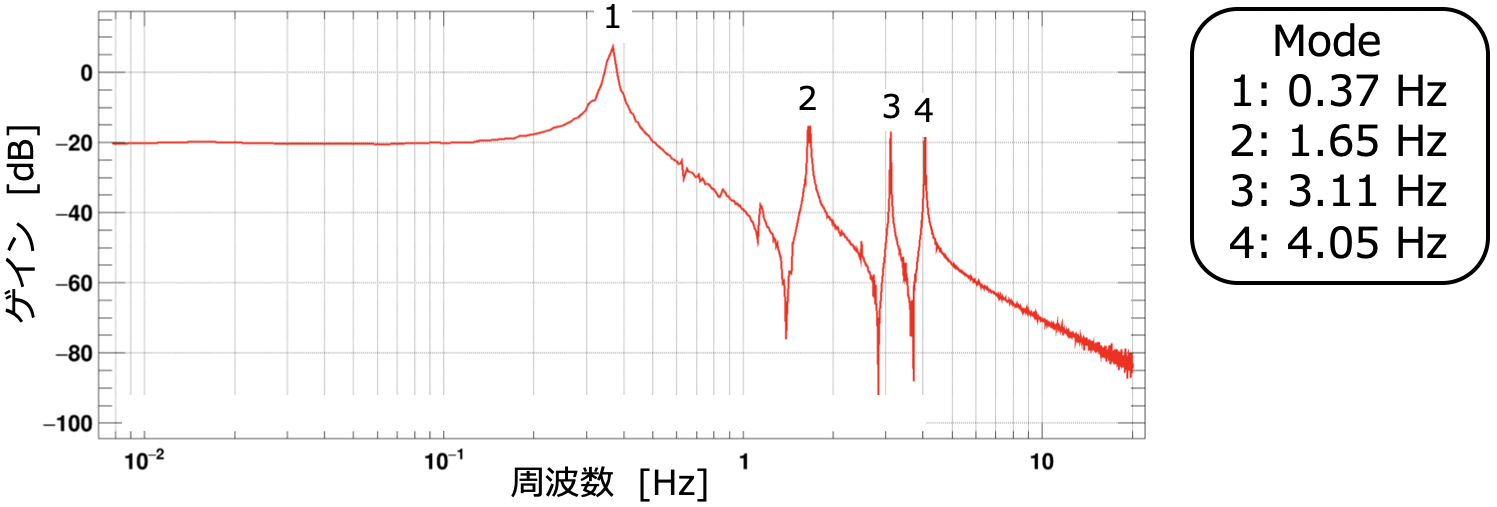
\includegraphics[width=150mm]{figD_10.png}
\end{center}
\end{figure}
\noindent
\underline{{\bf ITMX MN L}}
\begin{figure}[H]
\begin{center}
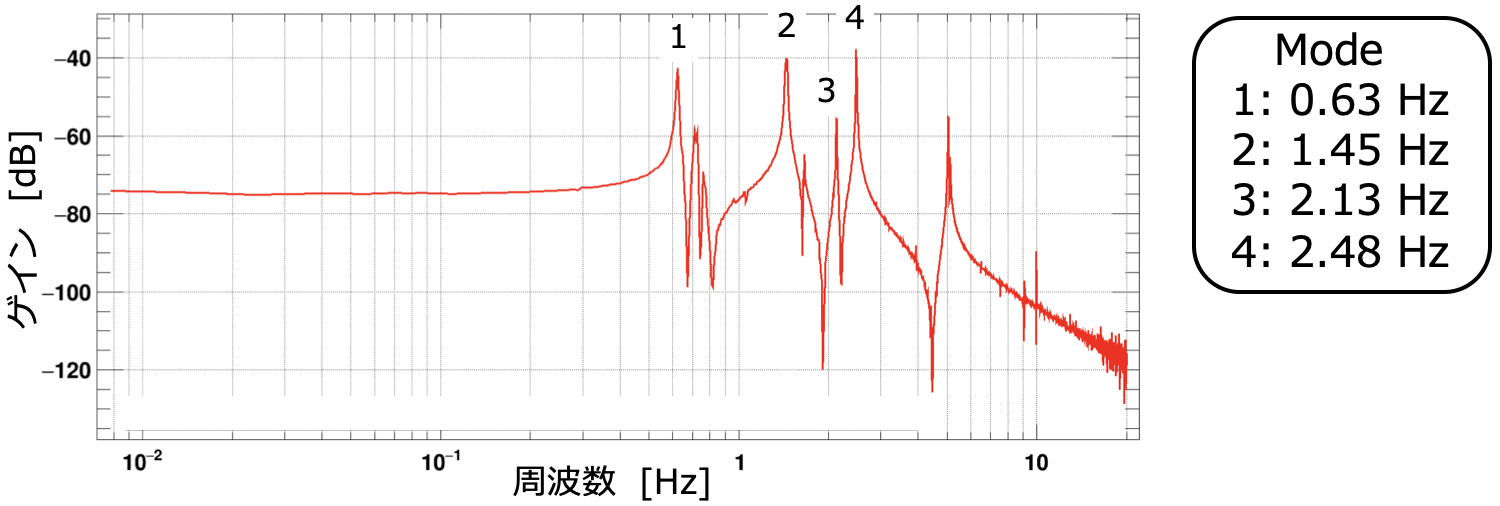
\includegraphics[width=150mm]{figD_11.png}
\end{center}
\end{figure}
\clearpage
\noindent
\underline{{\bf ITMX MN T}}
\begin{figure}[H]
\begin{center}
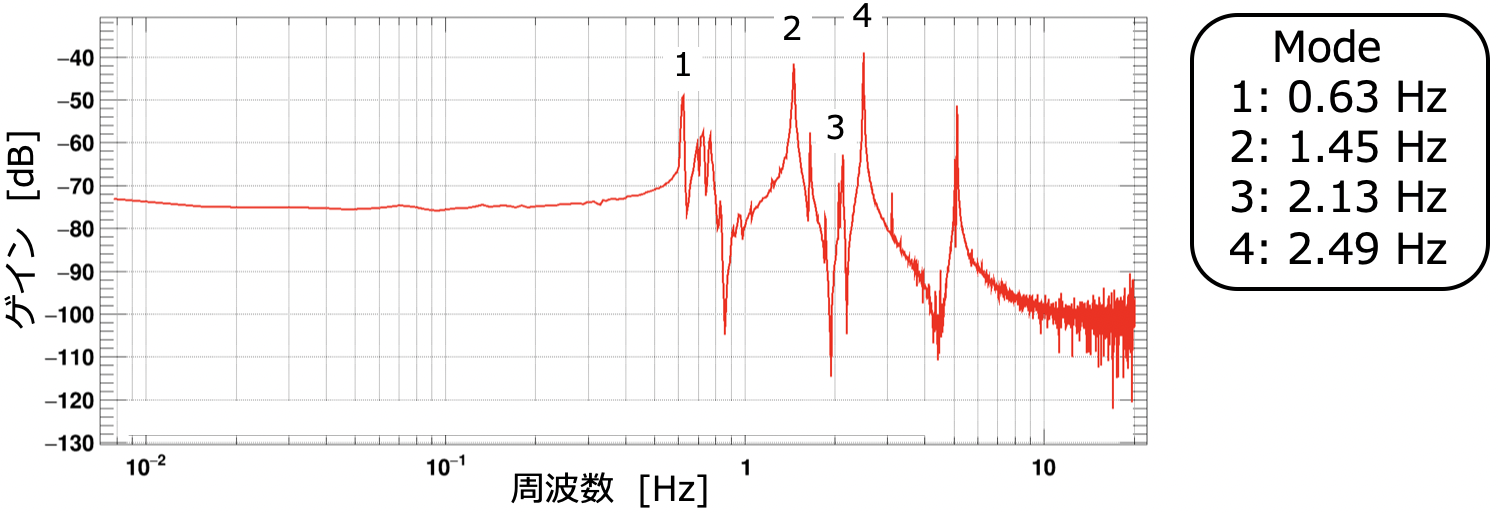
\includegraphics[width=150mm]{figD_12.png}
\end{center}
\end{figure}
\noindent
\underline{{\bf ITMX MN R}}
\begin{figure}[H]
\begin{center}
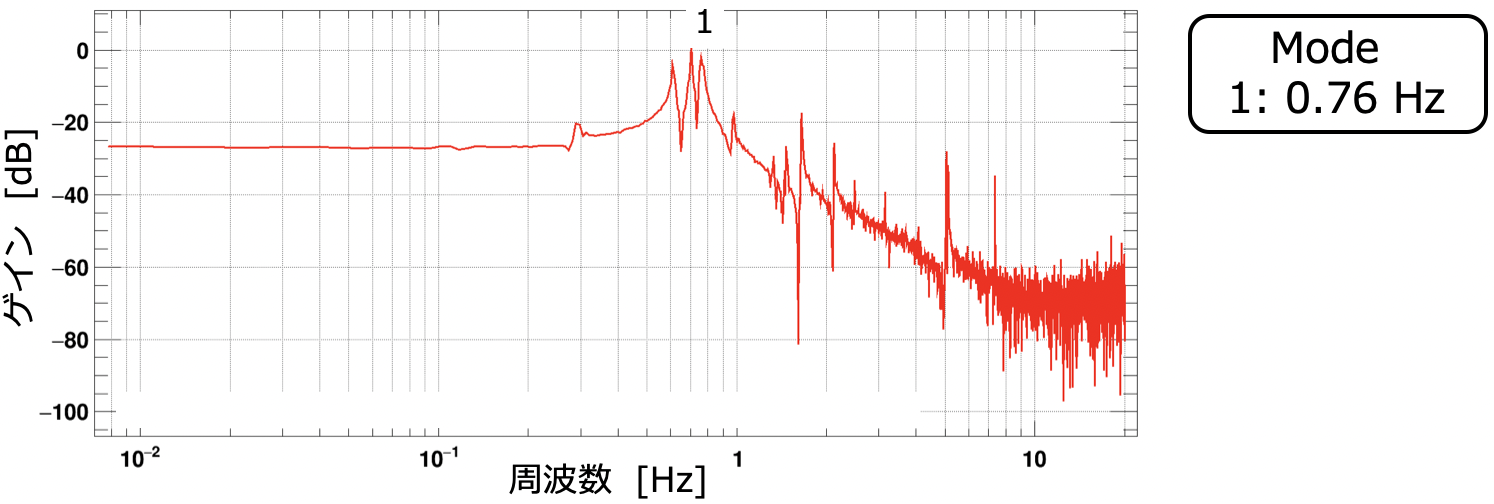
\includegraphics[width=150mm]{figD_13.png}
\end{center}
\end{figure}
\noindent
\underline{{\bf ITMX MN P}}
\begin{figure}[H]
\begin{center}
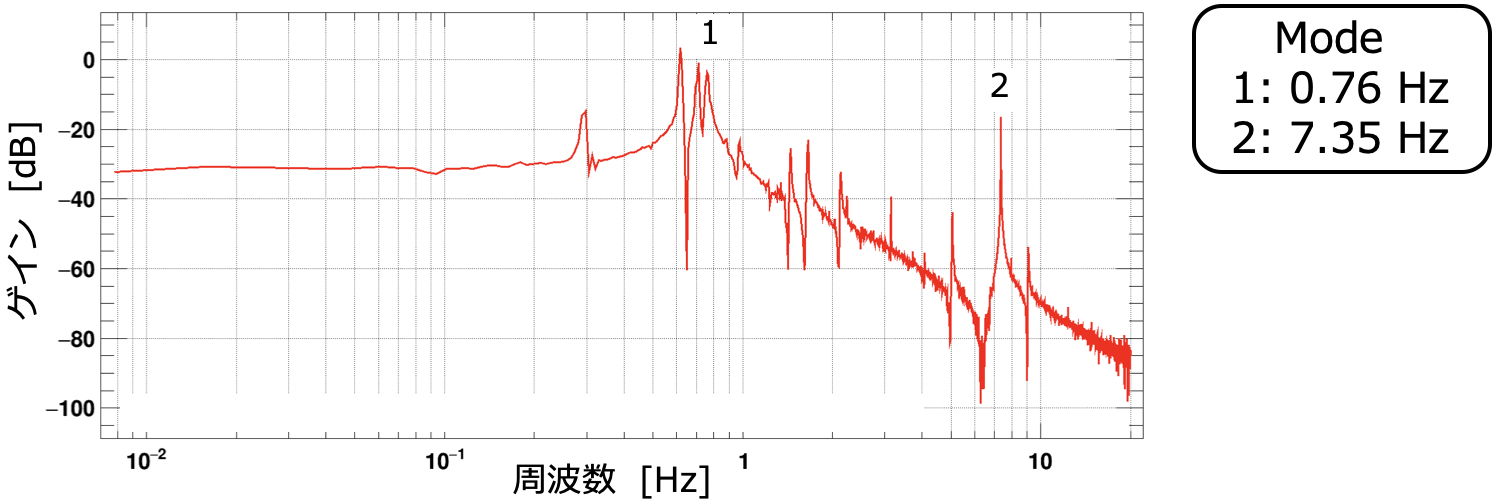
\includegraphics[width=150mm]{figD_14.png}
\end{center}
\end{figure}
\clearpage
\noindent
\underline{{\bf ITMX MN Y}}
\begin{figure}[H]
\begin{center}
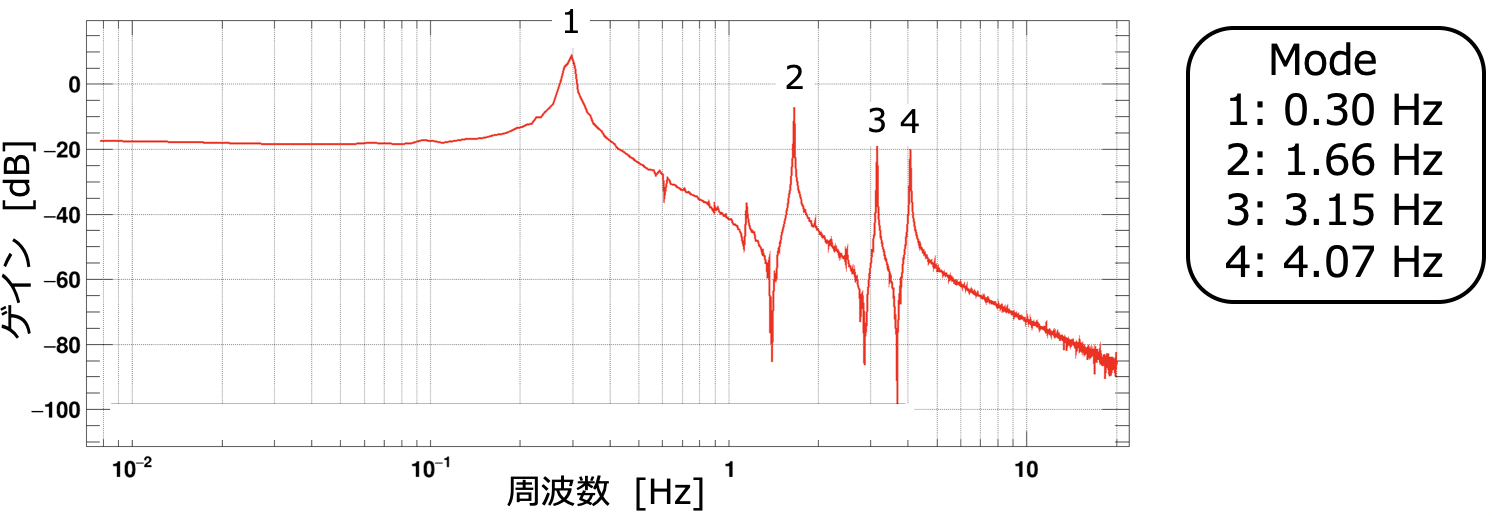
\includegraphics[width=150mm]{figD_15.png}
\end{center}
\end{figure}
\noindent
\underline{{\bf ITMY MN L}}
\begin{figure}[H]
\begin{center}
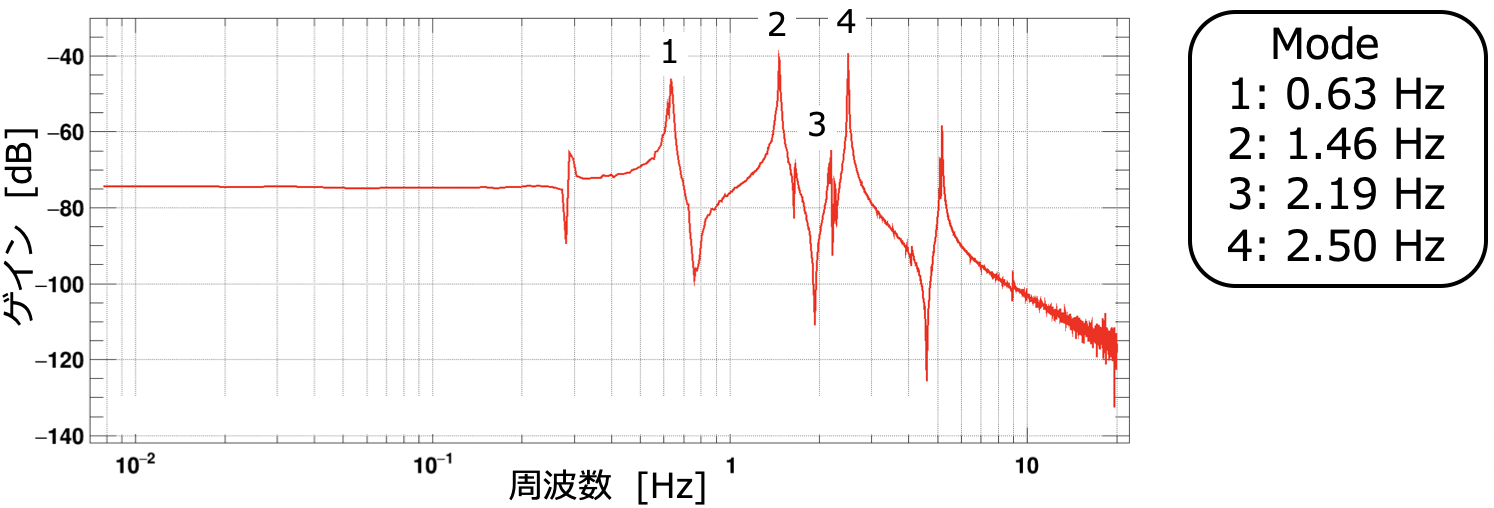
\includegraphics[width=150mm]{figD_16.png}
\end{center}
\end{figure}
\noindent
\underline{{\bf ITMY MN T}}
\begin{figure}[H]
\begin{center}
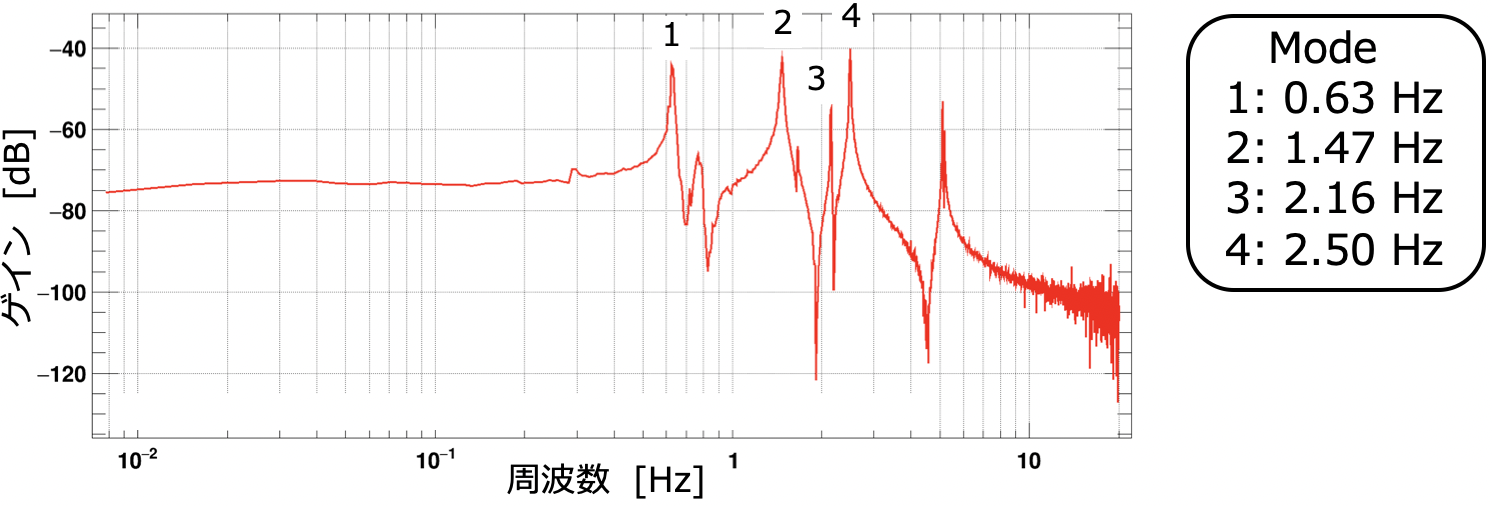
\includegraphics[width=150mm]{figD_17.png}
\end{center}
\end{figure}
\clearpage
\noindent
\underline{{\bf ITMY MN R}}
\begin{figure}[H]
\begin{center}
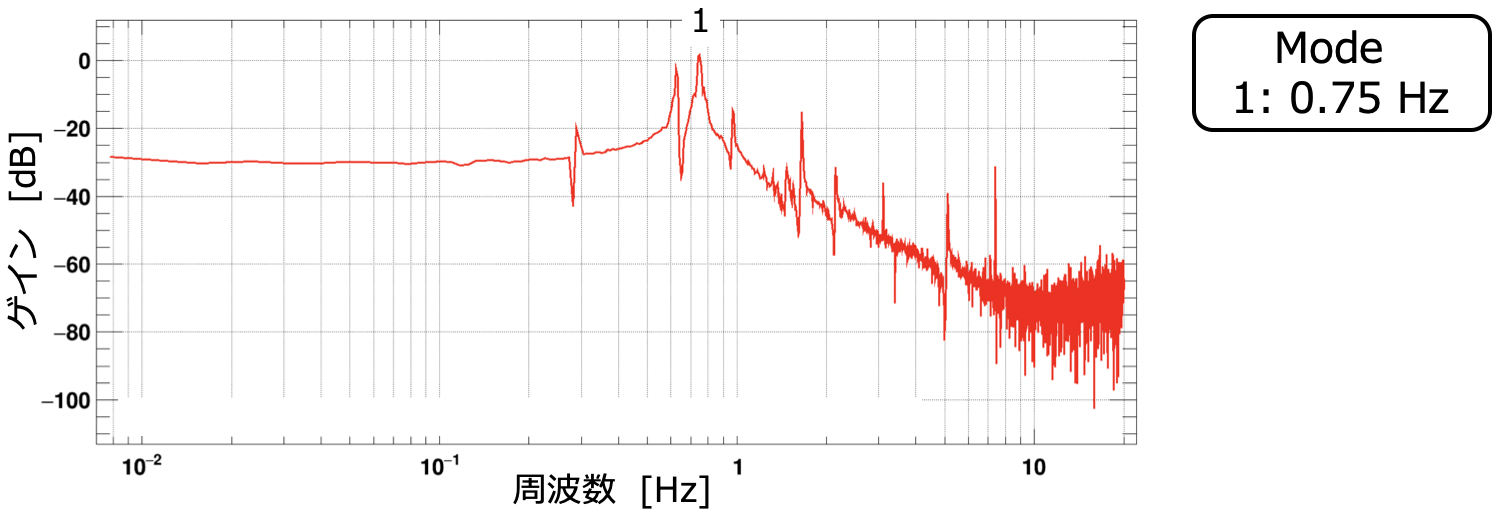
\includegraphics[width=150mm]{figD_18.png}
\end{center}
\end{figure}
\noindent
\underline{{\bf ITMY MN P}}
\begin{figure}[H]
\begin{center}
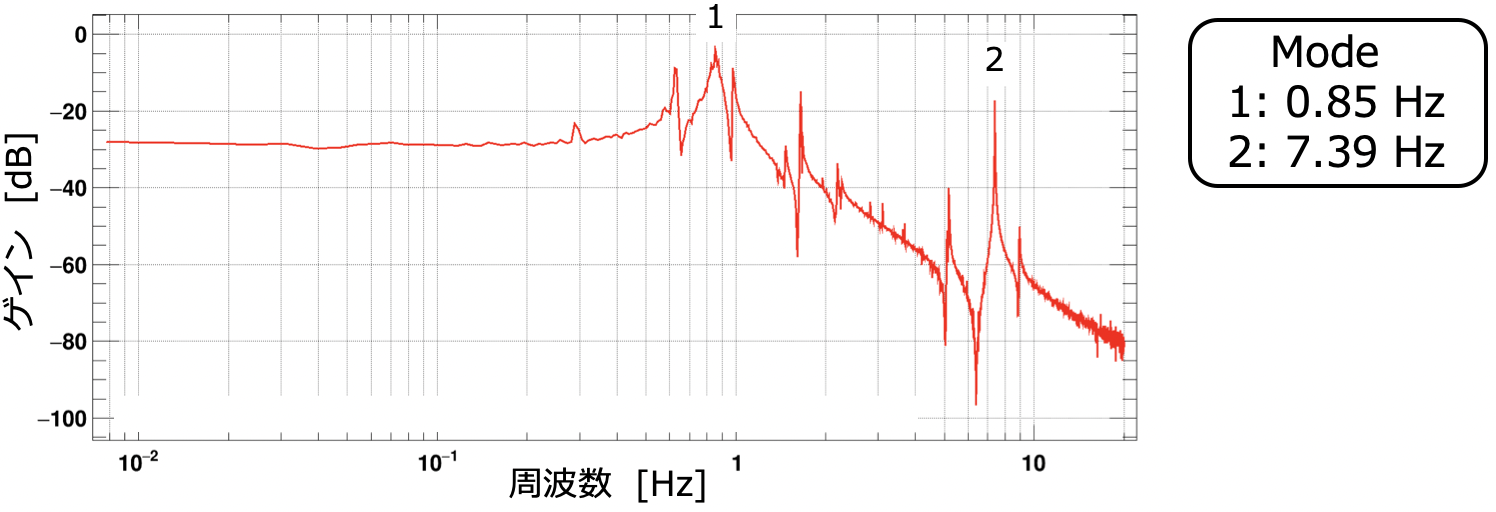
\includegraphics[width=150mm]{figD_19.png}
\end{center}
\end{figure}
\noindent
\underline{{\bf ITMY MN Y}}
\begin{figure}[H]
\begin{center}
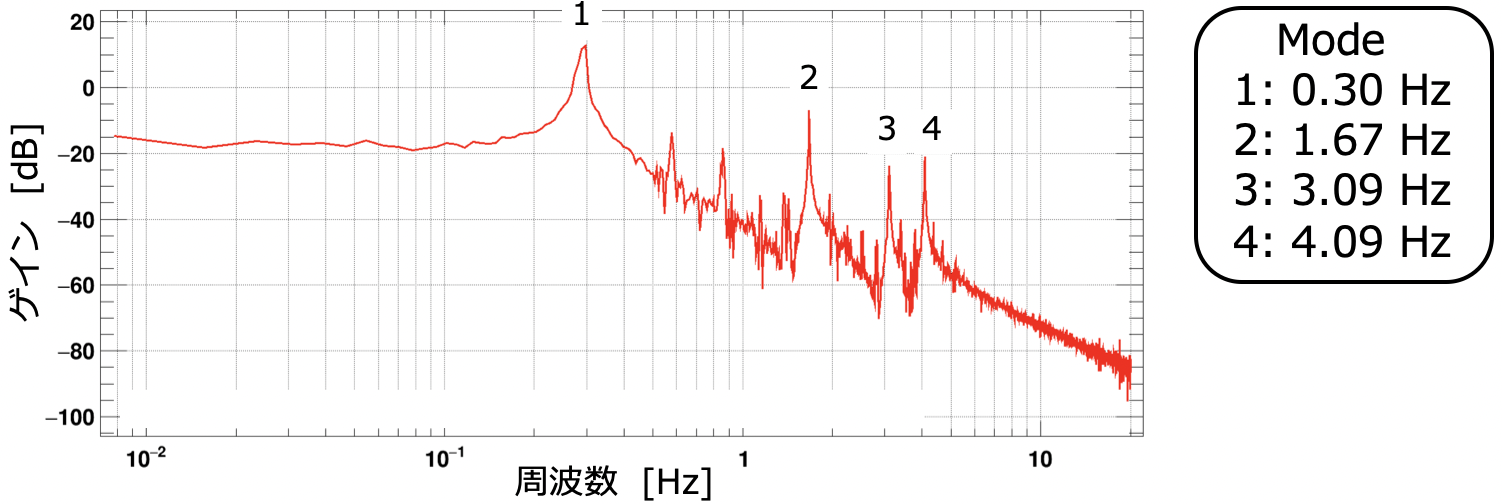
\includegraphics[width=150mm]{figD_20.png}
\end{center}
\end{figure}